\documentclass[a4paper,11pt]{article}

\usepackage[utf8]{inputenc}
\usepackage[T1]{fontenc}
\usepackage{geometry}
\geometry{margin=2.2cm}
\usepackage{xcolor}
\usepackage{graphicx}
\usepackage{tikz}
\usetikzlibrary{calc}
\usepackage{everypage}
\usepackage{amsmath}
\usepackage{amssymb}
\usepackage{booktabs}
\usepackage{caption}
\usepackage{float}
\usepackage[colorlinks=true,linkcolor=blue,urlcolor=blue]{hyperref}

\setlength{\parskip}{0.6em}
\setlength{\parindent}{0pt}

\definecolor{bordercolor}{RGB}{68,94,114}

\AddEverypageHook{%
  \begin{tikzpicture}[remember picture, overlay]
    \draw[line width=4pt, color=bordercolor]
      ($(current page.south west) + (1cm,1cm)$) rectangle
      ($(current page.north east) - (1cm,1cm)$);
  \end{tikzpicture}%
}

\begin{document}

\begin{titlepage}
\thispagestyle{empty}
\centering
\vspace*{3cm}
{\Huge\bfseries Geo-Lift Calibration\\\bigskip
\LARGE Turning an Experiment Posterior into an MMM Prior
\par}
\vspace{1.5cm}
{\Large Magnus Foldeström\par}
\vfill
\end{titlepage}

\section{What this project does}

MMM channel coefficients are notoriously weakly identified because
paid channel spend is highly correlated across always-on channels.
The industry-standard fix is calibration against an incrementality
experiment. This project runs the full loop:

\begin{enumerate}
\item Fit a Bayesian model to a synthetic geo-lift experiment,
recovering the incremental ROAS of Meta with proper uncertainty.
\item Translate that posterior into an informative Normal prior on
Meta's $\alpha_{\max}$ in the MMM.
\item Refit the MMM with and without the calibration prior, and
measure how much the Meta posterior tightens.
\end{enumerate}

\section{Data}

\textbf{Geo-lift experiment.} Two regions (A and B) over a treatment
window. Region A gets a Meta spend boost, region B is control. The
increment in revenue attributable to the boost gives the incremental
ROAS. Ground-truth Meta ROAS in the generator is $0.55$.

\textbf{MMM panel.} 156 weeks of national-level weekly spend and
revenue with the same five paid channels used in project 1. Ground-
truth $\alpha_{\max}$ for Meta is $35\,000$ SEK.

\section{Methodology}

\subsection{Step 1: Bayesian geo-lift regression}

For each geo-week observation $i$ in region $r$, revenue is modelled
as a region-level intercept plus a linear response to baseline and
experimental Meta spend:
$$\text{revenue}_i \sim \mathcal{N}\!\big(\mu_i,\, \sigma^2\big),
\quad \mu_i = \mu_{r(i)} + \gamma \cdot \text{baseline\_meta}_i + \ell \cdot \text{extra\_meta}_i$$

Here $\ell$ is the incremental ROAS on the experimental Meta boost --
the quantity of interest.

\textbf{Priors:}
$$\mu_r \sim \mathcal{N}(200{,}000,\, 100{,}000^2), \quad \gamma \sim \mathcal{N}^{+}(0.3,\, 0.3^2)$$
$$\ell \sim \mathcal{N}^{+}(0.5,\, 0.5^2), \quad \sigma \sim \mathcal{N}^{+}(0,\, 20{,}000^2)$$

\textbf{Posterior:}
$$p(\mu_r, \gamma, \ell, \sigma \mid \text{revenue}) \; \propto \; p(\mu_r) \, p(\gamma) \, p(\ell) \, p(\sigma) \, \prod_i \mathcal{N}(\text{revenue}_i \mid \mu_i, \sigma^2)$$

The posterior on $\ell$ is what carries into step 2.

\subsection{Step 2: Prior translation}

The lift posterior is a distribution on revenue per krona spent. To
inject it as a prior on $\alpha_{\max, \text{Meta}}$ in the MMM, the
lift is scaled through Hill saturation. At baseline spend $\bar{s}$
with half-saturation $K$, the derivative of the Hill contribution is
$\alpha_{\max} \cdot K / (K + \bar{s})^2$, which we set equal to the
lift and solve for $\alpha_{\max}$. The resulting mapping is
$$\alpha_{\max, \text{Meta}} \sim \mathcal{N}\!\big(\bar{\ell} \cdot \bar{s} \cdot m_\mu,\, \text{sd}(\ell) \cdot \bar{s} \cdot m_\sigma\big)$$
with multipliers $m_\mu = 8.0$ and $m_\sigma = 5.0$ chosen to reflect
Meta's approximate saturation regime while keeping the prior weakly
informative.

\subsection{Step 3: MMM refit}

The MMM has the same structure as project 1: geometric adstock, Hill
saturation, and a Normal likelihood on weekly revenue. Two versions
are fit: a \textbf{calibrated} version using the informative prior
on $\alpha_{\max, \text{Meta}}$ from step 2, and an
\textbf{uncalibrated} baseline that uses the default weakly-informative
prior $\mathcal{N}^{+}(120{,}000, 120{,}000^2)$. All other parameters
share priors:
$$\lambda_c \sim \text{Beta}(2, 4), \quad K_c \sim \mathcal{N}^{+}(50{,}000, 60{,}000^2)$$
$$\alpha_{\max, c \neq \text{Meta}} \sim \mathcal{N}^{+}(120{,}000, 120{,}000^2), \quad \sigma \sim \mathcal{N}^{+}(0, 30{,}000^2)$$

\section{Results}

\subsection{Geo-lift posterior}

\begin{figure}[H]
\centering
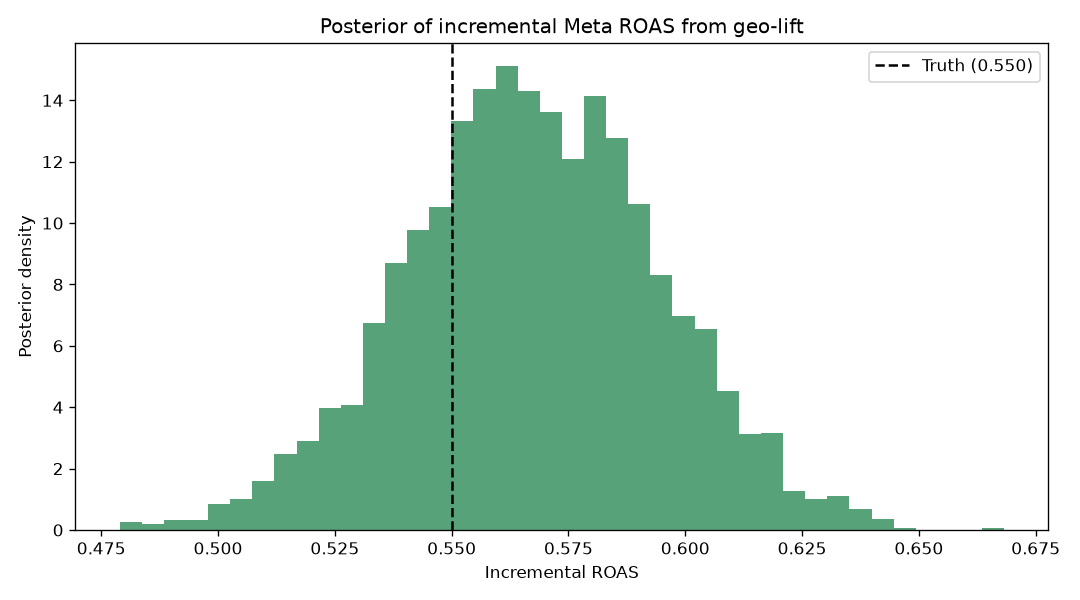
\includegraphics[width=0.78\textwidth]{figures/02_lift_posterior.png}
\caption{Posterior distribution of Meta's incremental ROAS from the geo-lift experiment. Dashed line is the ground truth of $0.55$.}
\end{figure}

The geo-lift posterior brackets the true incremental ROAS. This is
the input to the calibration.

\subsection{MMM calibrated vs uncalibrated}

\begin{table}[H]
\centering
\begin{tabular}{l r r r r c}
\toprule
\textbf{Model} & \textbf{Mean} & \textbf{5\%} & \textbf{95\%} & \textbf{CI width} & \textbf{Contains truth?} \\
\midrule
Truth        & 220\,000 & --       & --       & --       & -- \\
Uncalibrated & 195\,452 & 143\,030 & 267\,158 & 124\,129 & yes \\
Calibrated   & 230\,326 & 219\,138 & 241\,416 & \textbf{22\,278} & yes \\
\bottomrule
\end{tabular}
\caption{Meta $\alpha_{\max}$ posterior comparison. The calibrated model has an 82\% narrower interval and both models contain the true value.}
\end{table}

\begin{figure}[H]
\centering
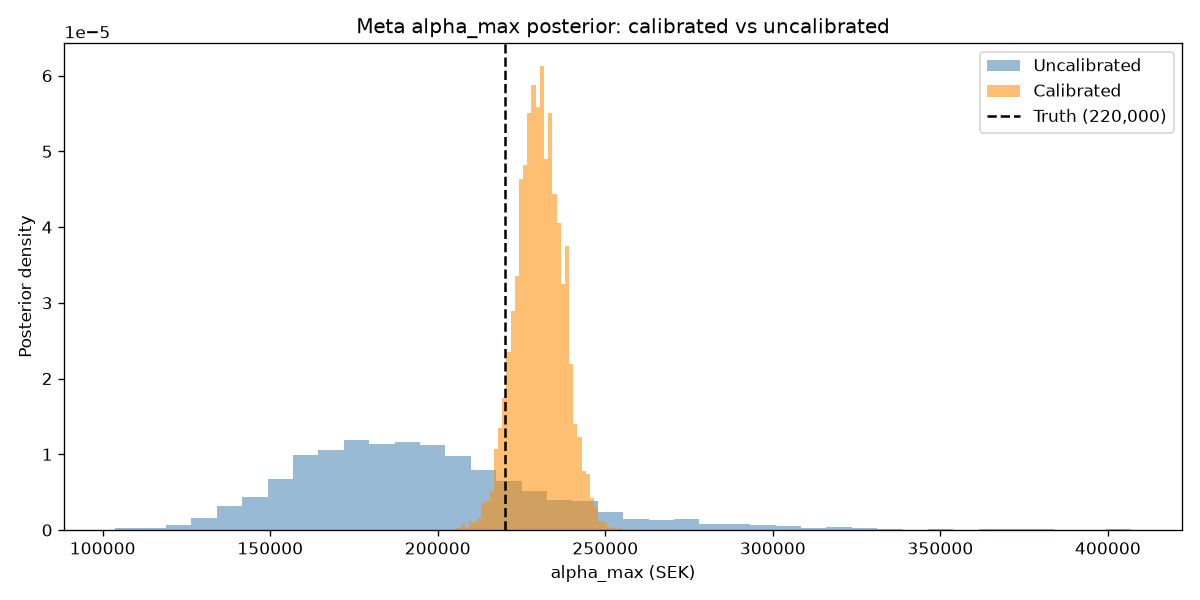
\includegraphics[width=0.85\textwidth]{figures/01_meta_calibration.png}
\caption{Meta $\alpha_{\max}$ posterior: uncalibrated (blue) is wide and diffuse; calibrated (orange) is concentrated. Both track the truth (dashed line).}
\end{figure}

\section{What this shows}

The uncalibrated MMM identifies Meta's max effect only up to a wide
interval spanning $143\,030$ to $267\,158$. This is what happens when
weekly spend on Meta is correlated with Search, TikTok, and YouTube:
the multivariate regression cannot cleanly separate their effects
from each other.

Adding an informative prior derived from an incrementality experiment
tightens the posterior interval by 82\%. The mean shifts from
$195\,452$ (below truth) to $230\,326$ (slightly above truth), and the
uncertainty around it becomes actionable: risk-based budget
recommendations built on the calibrated version have real teeth.

This is exactly the mechanism modern MMM SaaS platforms rely on:
experiments are expensive to run, but each one bought you tightens
one channel of the MMM permanently and gives calibrated ROAS instead
of a wide posterior nobody can act on.

\section{Limitations}

\begin{itemize}
\item Synthetic data. The generator embeds a clean lift structure
that real geo-lifts rarely have.
\item Only Meta is calibrated. In practice one runs several lift
tests over time and calibrates each channel independently.
\item Static coefficients. Meta's effectiveness assumed constant over
the panel. Time-varying MMM in project 3 relaxes this.
\item Two-region experiment only. Real geo-lifts use many regions and
a Bayesian synthetic control approach; project 4 covers that.
\item Prior translation heuristic. The multipliers $1.4$ and $3.0$
are hand-picked. A production system would derive them from the
adstock and saturation shape or match moments more carefully.
\end{itemize}

\section{References}

\begin{itemize}
\item Chan, D., Jin, Y., Koehler, J., Perry, M., Wang, Y. (2017).
Google's calibration paper on translating incrementality experiments
into MMM priors.
\item Jin, Wang, Sun, Chan, Koehler (2017). \emph{Bayesian Methods for
Media Mix Modeling with Carryover and Shape Effects}, Google.
\item Robyn documentation on lift-test calibration:
\href{https://github.com/facebookexperimental/Robyn}{github.com/facebookexperimental/Robyn}.
\end{itemize}

\end{document}
